% main.tex
% Last reviewed: 9 Oct 2024 by Sina Abdipoor
% WHAT ARE YOU DOING HERE? GO READ THE DAMN README!
% This is the main file. All the information for the thesis is gathered here. Also, all the formatting and margins are dealt with here as well.
\documentclass[openany, a4paper, 12pt, doublespacing]{book}
\usepackage{setspace, geometry, titlesec, fancyhdr, enumitem, graphicx, acro, color, makecell, amsmath, amsfonts, pifont, tabularx, hyperref}

\usepackage[style=apa, backend=biber]{biblatex}
\addbibresource{references.bib}
\addbibresource{publications.bib}

\usepackage{} % Add your packages here if needed

\graphicspath{{./figures/}} % Add all your figures to the "figures" folder.

% info.tex
% Last reviewed: 9 Oct 2024 by Sina Abdipoor
% TODO: Fill out your information in the second brackets {}. The data will automatically be reflected in all necessary parts of the thesis.

% Title of your thesis
\newcommand{\infothesistitle}{Title of Thesis}

% Your name
\newcommand{\infostudentname}{Name of Student}

% Your pronoun
\newcommand{\infostudentpronoun}{his}

% Your degree (eg. Doctor of Philosophy)
\newcommand{\infodegreename}{Name of Degree}

% Name of your faculty
\newcommand{\infofacultyname}{Name of Faculty}

% Year of your viva
\newcommand{\infovivayear}{Year}

% Month of your viva (eg. September)
\newcommand{\infovivamonth}{Month}

% Day of your viva
\newcommand{\infovivaday}{Day}

% Name of your supervisor
\newcommand{\infosupervisorname}{Name of Chairman of Supervisory Committee}

% Degree of your supervisor (leave empty if not applicable)
\newcommand{\infosupervisordegree}{, PhD}

% Title of your supervisor
\newcommand{\infosupervisortitle}{Title (e.g., Professor/Associate Professor/Ir; if applicable)}

% Faculty of your supervisor
\newcommand{\infosupervisorfaculty}{Name of Faculty}

% Name of your committee 1
\newcommand{\infocommitteeonename}{Name of Member 1}

% Degree of your committee 1 (leave empty if not applicable)
\newcommand{\infocommitteeonedegree}{, PhD}

% Title of your committee 1
\newcommand{\infocommitteeonetitle}{Title (e.g., Professor/Associate Professor/Ir; if applicable)}

% Faculty of your committee 1
\newcommand{\infocommitteeonefaculty}{Name of Faculty}

% Name of your committee 2
\newcommand{\infocommitteetwoname}{Name of Member 2}

% Degree of your committee 2 (leave empty if not applicable)
\newcommand{\infocommitteetwodegree}{, PhD}

% Title of your committee 2
\newcommand{\infocommitteetwotitle}{Title (e.g., Professor/Associate Professor/Ir; if applicable)}

% Faculty of your committee 2
\newcommand{\infocommitteetwofaculty}{Name of Department and/or Faculty}

% University of your committee 2
\newcommand{\infocommitteetwouniversity}{Name of Organisation (University / Institute)}

% Name of your committee 3 (leave the second bracket empty if you only have 3 members)
\newcommand{\infocommitteethreename}{Name of Member 3}

% Degree of your committee 3 (delete if not applicable) (leave the second bracket empty if you only have 3 members)
\newcommand{\infocommitteethreedegree}{, PhD}

% Title of your committee 3 (leave the second bracket empty if you only have 3 members)
\newcommand{\infocommitteethreetitle}{Title (e.g., Professor/Associate Professor/Ir; if applicable)}

% Faculty of your committee 3 (leave the second bracket empty if you only have 3 members)
\newcommand{\infocommitteethreefaculty}{Name of Department and/or Faculty}

% University of your committee 3 (leave the second bracket empty if you only have 3 members)
\newcommand{\infocommitteethreeuniversity}{Name of Organisation (University / Institute)}

% Abstract of your thesis
\newcommand{\infoabstractenglish}{The abstract is a digest of the entire thesis and should be given the same consideration as the main text. It does not normally include any reference to the literature. Abbreviations or acronyms must be preceded by the full term at the first use.

An abstract should be between 300-500 words. It includes a brief statement of the problem, a concise description of the research method and design, a summary of major findings, including their significance or lack of it, and conclusions.}

% Keywords of your thesis
\newcommand{\infokeywords}{Not more than 5 keywords in alphabetical order must be provided to describe the content of the thesis}

% SDG
\newcommand{\infosdg}{GOAL 4: Quality Education (as an example) - Not more than 3 goal}

% Title of your thesis in Malay
\newcommand{\infothesistitlemalay}{Tajuk Tesis}

% Name of your degree in Malay
\newcommand{\infodegreenamemalay}{Nama Ijazah}

% Month and year of your viva in Malay
\newcommand{\infovivadatemalay}{Bulan Tahun}

% Name of your faculty in Malay
\newcommand{\infofacultynamemalay}{Nama Fakulti}

% Abstract of your thesis in Malay
\newcommand{\infoabstractmalay}{Abstrak merupakan ringkasan keseluruhan tesis dan wajib diberi perhatian rapi sepertimana bahagian tesis yang lain. Abstrak tidak mengandungi bahan rujukan. Nama singkatan atau akronim mesti didahului dengan terminology penuh pada penggunaan kali pertama.

Abstrak harus diolah antara 300-500 perkataan. Abstrak merangkumi pernyataan permasalahan, penerangan rigkas dan tepat tentang reka bentuk dan pengkaedahan penyelidikan, rumusan penemuan utama dan kesimpulan.}

% Keywords in Malay
\newcommand{\infokeywordsmalay}{Tidak lebih daripada 5 kata kunci dalam susunan abjad perlu disediakan untuk menerangkan kandungan tesis}

% SDG in Malay
\newcommand{\infosdgmalay}{MATLAMAT 4: Pendidikan Berkualiti (sebagai contoh) – Tidak lebih dari 3 matlamat}

% Your acknowledgments
\newcommand{\infoacks}{Acknowledgements are written expressions of appreciation for guidance and assistance received from individuals and institutions.}

% Name of the chairperson of the examination committee
\newcommand{\infochairpersonname}{Name of Chairperson}

% Degree of the chairperson of the examination committee (leave empty if not applicable)
\newcommand{\infochairpersondegree}{, PhD}

% Title of the chairperson of the examination committee
\newcommand{\infochairpersontitle}{Title (e.g., Professor/Associate Professor/Ir; omit if irrelevant)}

% Faculty of the chairperson of the examination committee
\newcommand{\infochairpersonfaculty}{Name of Faculty}

% Name of the examiner 1 of the examination committee
\newcommand{\infoexamineronename}{Name of Examiner 1}

% Degree of the examiner 1 of the examination committee (leave empty if not applicable)
\newcommand{\infoexamineronedegree}{, PhD}

% Title of the examiner 1 of the examination committee
\newcommand{\infoexamineronetitle}{Title (e.g., Professor/Associate Professor/Ir; omit if irrelevant)}

% Faculty of the examiner 1 of the examination committee
\newcommand{\infoexamineronefaculty}{Name of Faculty}

% Name of the examiner 2 of the examination committee
\newcommand{\infoexaminertwoname}{Name of Examiner 2}

% Degree of the examiner 2 of the examination committee (leave empty if not applicable)
\newcommand{\infoexaminertwodegree}{, PhD}

% Title of the examiner 2 of the examination committee
\newcommand{\infoexaminertwotitle}{Title (e.g., Professor/Associate Professor/Ir; omit if irrelevant)}

% Faculty of the examiner 2 of the examination committee
\newcommand{\infoexaminertwofaculty}{Name of Faculty}

% Name of the external examiner of the examination committee
\newcommand{\infoexternalexaminername}{Name of External Examiner}

% Degree of the external examiner of the examination committee (leave empty if not applicable)
\newcommand{\infoexternalexaminerdegree}{, PhD}

% Title of the external examiner of the examination committee
\newcommand{\infoexternalexaminertitle}{Title (e.g., Professor/Associate Professor/Ir; omit if irrelevant)}

% Department and faculty of the external examiner of the examination committee
\newcommand{\infoexternalexaminerdepartment}{Name of Department and/or Faculty}

% University of the external examiner of the examination committee
\newcommand{\infoexternalexamineruniversity}{Name of Organisation (University/Institute)}

% Country of the external examiner of the examination committee
\newcommand{\infoexternalexaminercountry}{Country}

% Name of current Dean
\newcommand{\infodeanname}{Current Dean Name}

% Degree of the current Dean (leave empty if not applicable)
\newcommand{\infodeandegree}{, PhD}

% Name of current Deputy Dean
\newcommand{\infodeputydeanname}{Current Deputy Dean Name}

% Degree of the current Deputy Dean (leave empty if not applicable)
\newcommand{\infodeputydeandegree}{, PhD}

% Your Biodata
\newcommand{\infostudentbiodata}{This section is compulsory. It contains the student’s biographical information, such as name, educational background, the degree that is being sought, professional work experience (if any), and any other similar matters that may interest the reader. The vita should be in essay form, rather than a mere résumé.}
% acronym.tex
% Last reviewed: 3 Oct 2024 by Sina Abdipoor
% TODO: Define all your abbreviations here, as shown below. When writing your thesis, you can use them with the "\ac{}" command. For example: "I don't know why I decided to study at \ac{UPM}." LaTeX will automatically use the long version the first time and the short version thereafter. Additionally, all your abbreviations will be included in the table of abbreviations.
\DeclareAcronym{upm}{
  short=UPM,
  long=Universiti Putra Malaysia,
}

% Formatting starts here
%\geometry{top=2.33cm, bottom=2.22cm, left=2.29cm, right=0.81cm}
\geometry{top=2.33cm, bottom=2.22cm}

\setlength{\parindent}{0pt}
\setlength{\parskip}{\baselineskip}

\pagestyle{fancy}
\fancyhf{}
\fancyfoot[C]{\thepage}
\renewcommand{\headrulewidth}{0pt}

\setcounter{secnumdepth}{3}

\makeatletter
\renewcommand{\@dotsep}{1000}
\makeatother

\titleformat{\chapter}[display]{\normalsize\bfseries\centering}{CHAPTER \thechapter}{1em}{\uppercase}
\titleformat{\section}{\normalsize\bfseries}{\thesection}{1em}{}
\titleformat{\subsection}{\normalsize\bfseries}{\thesubsection}{1em}{}
\titleformat{\subsubsection}{\normalsize\bfseries}{\thesubsubsection}{1em}{}
\titlespacing{\chapter}{0pt}{0pt}{0pt}
\titlespacing{\section}{0pt}{0pt}{0pt}
\titlespacing{\subsection}{0pt}{0pt}{0pt}
\titlespacing{\subsubsection}{0pt}{0pt}{0pt}
% Formatting ends here

\begin{document}

\begin{titlepage}
    \begin{singlespace}
        % titlepage.tex
% Last reviewed: 9 Oct 2024 by Sina Abdipoor
\begin{center}
    
\includegraphics[width=0.5\linewidth]{upm-logo.jpg} \\ \vspace{1cm}
    \textbf{\MakeUppercase{\infothesistitle}} \\ \vfill
    \textbf{By} \\ \vspace{1cm}
    \textbf{\MakeUppercase{\infostudentname}} \\ \vspace{6cm}
    \textbf{Thesis Submitted to the School of Graduate Studies, \\Universiti Putra Malaysia, in Fulfilment of the Requirements for the Degree of \infodegreename} \\ \vspace{2cm}
    \textbf{{\infovivayear} {\infovivamonth}}
\end{center}
        % copyright.tex
% Last reviewed: 5 Oct 2024 by Sina Abdipoor
\thispagestyle{empty}
All material contained within the thesis, including without limitation text, logos, icons, photographs and all other artwork, is copyright material of Universiti Putra Malaysia unless otherwise stated. Use may be made of any material contained within the thesis for non-commercial purposes from the copyright holder. Commercial use of material may only be made with the express, prior, written permission of Universiti Putra Malaysia.
    
\copyright{Universiti Putra Malaysia}
    \end{singlespace}
\end{titlepage}

\frontmatter
% abstract.tex
% Last reviewed: 3 Oct 2024 by Sina Abdipoor
\addcontentsline{toc}{chapter}{ABSTRACT}
\begin{center}
    \begin{singlespace}
        Abstract of thesis presented to the Senate of Universiti Putra Malaysia in fulfilment of the requirement for the degree of \infodegreename
    \end{singlespace}

    \textbf{\MakeUppercase{\infothesistitle}}

    By \\
    \textbf{\MakeUppercase{\infostudentname}}

    \textbf{{\infovivamonth} {\infovivayear}}
\end{center}

\begin{tabular}{ll}
\textbf{Chairman} & \textbf{: \infosupervisorname \infosupervisordegree} \\
\textbf{Faculty} & \textbf{: \infofacultyname}
\end{tabular}

\infoabstractenglish

\begin{singlespace}
    \textbf{Keywords:} \infokeywords
    
    \textbf{SDG:} \infosdg
\end{singlespace}
% abstrak.tex
% Last reviewed: 3 Oct 2024 by Sina Abdipoor
\addcontentsline{toc}{chapter}{ABSTRAK}
\begin{center}
    \begin{singlespace}
        Abstrak tesis yang dikemukakan kepada Senat Universiti Putra Malaysia sebagai memenuhi keperluan untuk ijazah \infodegreenamemalay
    \end{singlespace}

    \textbf{\MakeUppercase{\infothesistitlemalay}}

    Oleh \\
    \textbf{\MakeUppercase{\infostudentname}}

    \textbf{\infovivadatemalay}
\end{center}

\begin{tabular}{ll}
\textbf{Pengerusi} & \textbf{: \infosupervisorname \infosupervisordegree} \\
\textbf{Fakulti} & \textbf{: \infofacultynamemalay}
\end{tabular}

\infoabstractmalay

\begin{singlespace}
    \textbf{Kata Kunci:} \infokeywordsmalay
    
    \textbf{SDG:} \infosdgmalay
\end{singlespace}
% acknowledgment.tex
% Last reviewed: 3 Oct 2024 by Sina Abdipoor
\chapter{ACKNOWLEDGMENTS}
\infoacks

\begin{singlespace}
    % approval.tex
% Last reviewed: 8 Oct 2024 by Sina Abdipoor
\addcontentsline{toc}{chapter}{APPROVAL}

I certify that a Thesis Examination Committee has met on {\infovivaday} {\infovivamonth} {\infovivayear} to conduct the final examination of {\infostudentname} on {\infostudentpronoun} thesis entitled “\infothesistitle” in accordance with the Universities and University Colleges Act 1971 and the Constitution of the Universiti Putra Malaysia [P.U.(A) 106] 15 March 1998. The Committee recommends that the student be awarded the \infodegreename.

Members of the Thesis Examination Committee were as follows:

\textbf{\infochairpersonname \infochairpersondegree} \\
\infochairpersontitle \\
\infochairpersonfaculty \\
Universiti Putra Malaysia \\
(Chairman)

\textbf{\infoexamineronename \infoexamineronedegree} \\
\infoexamineronetitle \\
\infoexamineronefaculty \\
Universiti Putra Malaysia \\
(Internal Examiner)

% Delete these 5 lines if you only have 1 internal examiner
\textbf{\infoexaminertwoname \infoexaminertwodegree} \\
\infoexaminertwotitle \\
\infoexaminertwofaculty \\
Universiti Putra Malaysia \\
(Internal Examiner)

\textbf{\infoexternalexaminername \infoexternalexaminerdegree} \\
\infoexternalexaminertitle \\
\infoexternalexaminerdepartment \\
\infoexternalexamineruniversity \\
\infoexternalexaminercountry \\
(External Examiner)

\begin{minipage}[t]{0.5\textwidth}
    \hfill
\end{minipage}
\begin{minipage}[t]{0.5\textwidth}
    \rule{6cm}{0.4pt} \\
    \textbf{\infodeputydeanname \infodeputydeandegree} \\
    Professor and Deputy Dean \\
    School of Graduate Studies \\
    Universiti Putra Malaysia \\

    Date:
\end{minipage}

\newpage

This thesis was submitted to the Senate of Universiti Putra Malaysia and has
been accepted as fulfilment of the requirement for the degree of \infodegreename. The members of the Supervisory Committee were as follows:

\textbf{\infosupervisorname \infosupervisordegree} \\
\infosupervisortitle \\
\infosupervisorfaculty \\
Universiti Putra Malaysia \\
(Chairman)

\textbf{\infocommitteeonename \infocommitteeonedegree} \\
\infocommitteeonetitle \\
\infocommitteeonefaculty \\
Universiti Putra Malaysia \\
(Member)

\textbf{\infocommitteetwoname \infocommitteetwodegree} \\
\infocommitteetwotitle \\
\infocommitteetwofaculty \\
\infocommitteetwouniversity \\
(Member)

% Delete these 5 lines if you only have 3 committee
\textbf{\infocommitteethreename \infocommitteethreedegree} \\
\infocommitteethreetitle \\
\infocommitteethreefaculty \\
\infocommitteethreeuniversity \\
(Member)

\begin{minipage}[t]{0.5\textwidth}
    \hfill
\end{minipage}
\begin{minipage}[t]{0.5\textwidth}
    \rule{6cm}{0.4pt} \\
    \textbf{\infodeanname \infodeandegree} \\
    Professor and Dean \\
    School of Graduate Studies \\
    Universiti Putra Malaysia \\

    Date:
\end{minipage}
    % declaration.tex
% Last reviewed: 9 Oct 2024 by Sina Abdipoor
\addcontentsline{toc}{chapter}{DECLARATION}

\textbf{Declaration by the Graduate Student}

\begin{minipage}{\linewidth}
   I hereby confirm that:
    \begin{itemize}[noitemsep, topsep=0pt, leftmargin=*]
        \item this thesis is my original work;
        \item quotations, illustrations and citations have been duly referenced;
        \item this thesis has not been submitted previously or concurrently for any other degree at any institutions;
        \item intellectual property from the thesis and the copyright of the thesis are fully-owned by Universiti Putra Malaysia, as stipulated in the Universiti Putra Malaysia (Research) Rules 2012;
        \item written permission must be obtained from the supervisor and the office of the Deputy Vice-Chancellor (Research and innovation) before the thesis is published in any written, printed or electronic form (including books, journals, modules, proceedings, popular writings, seminar papers, manuscripts, posters, reports, lecture notes, learning modules or any other materials) as stated in the Universiti Putra Malaysia (Research) Rules 2012;
        \item there is no plagiarism or data falsification/fabrication in the thesis, and scholarly integrity is upheld in accordance with the Universiti Putra Malaysia (Graduate Studies) Rules 2003 (Revision 2015-2016) and the Universiti Putra Malaysia (Research) Rules 2012. The thesis has undergone plagiarism detection software.
    \end{itemize} 
\end{minipage}

Signature: \rule{6cm}{0.4pt} Date: \hrulefill

Name and Matric No.: \hrulefill

\newpage

\textbf{Declaration by Members of the Supervisory Committee}

\begin{minipage}{\linewidth}
    This is to confirm that:
    \begin{itemize}[noitemsep, topsep=0pt, leftmargin=*]
        \item the research and the writing of this thesis were done under our supervision;
        \item supervisory responsibilities as stated in the Universiti Putra Malaysia (Graduate Studies) Rules 2003 (Revision 2015-2016) are adhered to.
    \end{itemize}
\end{minipage}

\begin{tabular}{ll}
    Signature: & \makebox[8cm]{\hrulefill} \\
    Name of Chairman of & \\
    Supervisory Committee: & \makebox[8cm]{\hrulefill} \\ \vspace{1cm}
    \\
    Signature: & \makebox[8cm]{\hrulefill} \\
    Name of Member of & \\
    Supervisory Committee: & \makebox[8cm]{\hrulefill} \\ \vspace{1cm}
    \\
    Signature: & \makebox[8cm]{\hrulefill} \\
    Name of Member of & \\
    Supervisory Committee: & \makebox[8cm]{\hrulefill} \\ \vspace{1cm}
    \\
    % Delete these 3 lines if you only have 3 committee
    Signature: & \makebox[8cm]{\hrulefill} \\
    Name of Member of & \\
    Supervisory Committee: & \makebox[8cm]{\hrulefill} \\
\end{tabular}
\end{singlespace}

\begin{singlespace}
    \setlength{\parskip}{0pt}
    \renewcommand{\contentsname}{TABLE OF CONTENTS}
    \tableofcontents
    \setlength{\parskip}{\baselineskip}
    \renewcommand{\listtablename}{LIST OF TABLES}
    \listoftables
    \addcontentsline{toc}{chapter}{LIST OF TABLES}
    \renewcommand{\listfigurename}{LIST OF FIGURES}
    \listoffigures
    \addcontentsline{toc}{chapter}{LIST OF FIGURES}
    \printacronyms[name=LIST OF ABBREVIATIONS]
    \addcontentsline{toc}{chapter}{LIST OF ABBREVIATIONS}
\end{singlespace}

\mainmatter
% thesis.tex
% Last reviewed: 9 Oct 2024 by Sina Abdipoor
% TODO: Start writing your thesis here. Make sure you read the README first.
\chapter{INTRODUCTION}
There may be a preamble at the beginning of a chapter. The purpose may be to introduce the themes of the main headings.

\section{Main heading no. 1 (Primary Level Numbering)}

\subsection{Subheading no. 1 (Secondary level numbering)}
There should be at least two subheadings to justify having subheadings.

\subsection{Subheading no. 2 (Secondary level numbering)}
All first letters of principal words are capitalised and the subheading is left justified.

\subsubsection{Tertiary heading no. 1 (Under Subheading no. 2)}
There should be at least two tertiary headings to justify having tertiary headings.

\subsubsection{Tertiary heading no. 2 (Under Subheading no. 2)}
Tertiary and subsequent headings should not be listed in the Table of Contents.

\newpage
\textcolor{blue}{Sample of Table (with vertical lines)}

\begin{table}[h]
%\centering
\renewcommand\cellalign{l}
\caption{Number of visitors according to participation in different activities}
\begin{tabular}{|l|c|c|}
    \hline
    \textbf{Activity} & \textbf{\makecell{No. of\\participants\\(N=96)}} & \textbf{NA} \\
    \hline
    Wildlife & - & 96 \\
    Sighting & - & 96 \\
    Fishing & 92 (95.8) & 4 \\
    Photography & - & 96 \\
    Camping & 47 (49.0) & 49 \\
    Picnicking & 96 (100) & - \\
    Visiting & 84 (87.5) & 12 \\
    Waterfall & 4 (4.2) & 92 \\
    \makecell{Sightseeing and nature\\observation} & 50 (52.1) & 46 \\
    \hline
\end{tabular}
\\Note: Figures in parentheses indicate percentage of N\\NA: Not applicable
\label{tab:visitor-count}
\end{table}

\newpage
\textcolor{blue}{Sample of Table (without vertical lines)}

\begin{table}[h]
%\centering
\caption{Number of visitors according to participation in different activities}
\begin{tabular}{lcc}
    \hline
    \textbf{Activity} & \textbf{\makecell{No. of participants\\(N=96)}} & \textbf{NA} \\
    \hline
    Wildlife & - & 96 \\
    Sighting & - & 96 \\
    Fishing & 92 (95.8) & 4 \\
    Photography & - & 96 \\
    Camping & 47 (49.0) & 49 \\
    Picnicking & 96 (100) & - \\
    Visiting & 84 (87.5) & 12 \\
    Waterfall & 4 (4.2) & 92 \\
    \hline
\end{tabular}
\\Note: Figures in parentheses indicate percentage of N\\NA: Not applicable\\(Source: \ac{upm})
\label{tab:visitor-count-2}
\end{table}

\newpage
\textcolor{blue}{Sample of Figure}

\begin{figure}[h]
    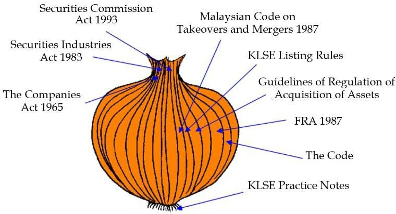
\includegraphics[width=0.75\linewidth]{onion.png}
    \caption{The Corporate Governance Framework in Malaysia—The Onion Model}
    (Source: \textcite{abdipoor2023meta} \tiny \textcolor{red}{not really}\normalsize)
    \label{fig:onion}
\end{figure}

\backmatter
\printbibliography[title={REFERENCES}]

\appendix
% appendix.tex
% Last reviewed: 3 Oct 2024 by Sina Abdipoor
% TODO: Write all your appendices here. Before removing the text below, read it to determine if and when you need an appendix. You can write here just as you would in the thesis.tex file, using \chapter, \section, references, etc. If you do not need an appendix in your thesis, go to main.tex and place a "%" before "% appendix.tex
% Last reviewed: 3 Oct 2024 by Sina Abdipoor
% TODO: Write all your appendices here. Before removing the text below, read it to determine if and when you need an appendix. You can write here just as you would in the thesis.tex file, using \chapter, \section, references, etc. If you do not need an appendix in your thesis, go to main.tex and place a "%" before "% appendix.tex
% Last reviewed: 3 Oct 2024 by Sina Abdipoor
% TODO: Write all your appendices here. Before removing the text below, read it to determine if and when you need an appendix. You can write here just as you would in the thesis.tex file, using \chapter, \section, references, etc. If you do not need an appendix in your thesis, go to main.tex and place a "%" before "\include{appendix}".
\chapter{APPENDICES}
Information or data that is too detailed for the main body of the thesis may be included as appendices. Appendices include original data, summary, sideline or preliminary tests, tabulations, tables that contain data of lesser importance, very lengthy quotations, supporting decisions, forms and documents, computer printouts, detailed engineering drawings and other pertinent documents. Appendix materials should be grouped by type, e.g., Appendix A: Questionnaire, Appendix B: Original data, Appendix C: Tables of results.".
\chapter{APPENDICES}
Information or data that is too detailed for the main body of the thesis may be included as appendices. Appendices include original data, summary, sideline or preliminary tests, tabulations, tables that contain data of lesser importance, very lengthy quotations, supporting decisions, forms and documents, computer printouts, detailed engineering drawings and other pertinent documents. Appendix materials should be grouped by type, e.g., Appendix A: Questionnaire, Appendix B: Original data, Appendix C: Tables of results.".
\chapter{APPENDICES}
Information or data that is too detailed for the main body of the thesis may be included as appendices. Appendices include original data, summary, sideline or preliminary tests, tabulations, tables that contain data of lesser importance, very lengthy quotations, supporting decisions, forms and documents, computer printouts, detailed engineering drawings and other pertinent documents. Appendix materials should be grouped by type, e.g., Appendix A: Questionnaire, Appendix B: Original data, Appendix C: Tables of results.
% biodata.tex
% Last reviewed: 9 Oct 2024 by Sina Abdipoor
\chapter{BIODATA OF STUDENT}
\infostudentbiodata

\begin{refsection}[publications.bib]
    \nocite{*}
    \printbibliography[title={LIST OF PUBLICATIONS}, heading=bibintoc]
\end{refsection}

\begin{singlespace}
    % confirmation.tex
% Last reviewed: 9 Oct 2024 by Sina Abdipoor
% I had to change pretty much everything (formatting, margins, etc.) for this one page because this page is totally different in the official template too.
% The coding of this page is absolutely disgusting and nasty. I just tried to make it match the official template as much as I could, not to mention this was the last page I did, and I was already so over it. I'm sure there are much better ways to implement this page. In case you feel like reimplementing it, you're more than welcome to do so. You could also send it to me to update the template.
\thispagestyle{empty}
\newgeometry{top=1cm, bottom=1cm, left=2cm, right=2cm}
\setlength{\parskip}{0.5\baselineskip}
\newcommand{\checkbox}{\scalebox{2}{\ding{113}}}
\small

\begin{center}
    
\includegraphics[width=0.25\linewidth]{upm-logo.jpg} \\
    \textbf{UNIVERSITI PUTRA MALAYSIA}
    
    \textbf{STATUS CONFIRMATION FOR THESIS / PROJECT REPORT AND COPYRIGHT}
    
    \textbf{ACADEMIC SESSION:} \rule{4cm}{0.4pt}
\end{center}

\textbf{TITLE OF THESIS / PROJECT REPORT:}

\hrulefill

\hrulefill

\hrulefill

\textbf{NAME OF STUDENT: } \rule{10cm}{0.4pt}

I acknowledge that the copyright and other intellectual property in the thesis/project report belonged to Universiti Putra Malaysia and I agree to allow this thesis/project report to be placed at the library under the following terms: \\

\begin{enumerate}[topsep=-0.5cm, leftmargin=*]
    \item This thesis/project report is the property of Universiti Putra Malaysia.
    \item The library of Universiti Putra Malaysia has the right to make copies for educational purposes only.
    \item The library of Universiti Putra Malaysia is allowed to make copies of this thesis for academic exchange. \\
\end{enumerate}

I declare that this thesis is classified as: \\
\footnotesize
\\\text{*}Please tick (\checkmark)

\begin{tabularx}{\textwidth}{@{}lX@{}}
    \checkbox \hspace{0.5cm} \textbf{CONFIDENTIAL} \hspace{2.5cm} & (Contain confidential information under Official Secret Act 1972). \\
    \checkbox \hspace{0.5cm} \textbf{RESTRICTED} & (Contains restricted information as specified by the organization/institution where research was done). \\
    \checkbox \hspace{0.5cm} \textbf{OPEN ACCESS} & I agree that my thesis/project report to be published as hard copy or online open access. \\
    The thesis is submitted for: & \\
    \checkbox \hspace{0.5cm} \textbf{PATENT} & Embargo from \rule{3cm}{0.4pt} until \rule{3cm}{0.4pt} \\
    & \hspace{3.4cm}(date) \hspace{3cm}(date)
\end{tabularx}

\footnotesize

\begin{minipage}[t]{0.5\textwidth}
    \hfill \\ \vspace{0.5cm}
    
    \rule{5cm}{0.4pt} \\
    (Signature of Student) \\
    New IC No/ Passport No.: \\

    Date:
\end{minipage}
\begin{minipage}[t]{0.5\textwidth}
    \textbf{Approved by:} \\ \vspace{0.5cm}
    
    \rule{5cm}{0.4pt} \\
    (Signature of Chairman of Supervisory Committee) \\
    Name: \\

    Date:
\end{minipage}

\textbf{[Note : If the thesis is CONFIDENTIAL or RESTRICTED, please attach with the letter from the organization/institution with period and reasons for confidentially or restricted.]}

\restoregeometry
\normalsize
\setlength{\parskip}{\baselineskip}
\end{singlespace}

\end{document}